% Figure 1: Method at a Glance — Pipeline Schematic
% Compile: pdflatex fig1_pipeline.tex
% Usage:   % Figure 1: Method at a Glance — Pipeline Schematic
% Compile: pdflatex fig1_pipeline.tex
% Usage:   % Figure 1: Method at a Glance — Pipeline Schematic
% Compile: pdflatex fig1_pipeline.tex
% Usage:   % Figure 1: Method at a Glance — Pipeline Schematic
% Compile: pdflatex fig1_pipeline.tex
% Usage:   \input{figures/fig1_pipeline} (without \documentclass wrapper)
\documentclass[border=8pt]{standalone}
\usepackage{tikz}
\usepackage{amsmath,amssymb}
\usetikzlibrary{
  arrows.meta,
  calc,
  positioning,
  decorations.pathreplacing,
  fit,
  backgrounds,
  shadows.blur,
  shapes.geometric,
  patterns
}

% ── Colour palette (monochrome + accent) ──
\definecolor{inputblue}{HTML}{2C3E50}
\definecolor{featureteal}{HTML}{1ABC9C}
\definecolor{backbonegray}{HTML}{5D6D7E}
\definecolor{headA}{HTML}{8E44AD}
\definecolor{headB}{HTML}{2980B9}
\definecolor{headC}{HTML}{2980B9}
\definecolor{projred}{HTML}{C0392B}
\definecolor{splineorg}{HTML}{D35400}
\definecolor{outputgrn}{HTML}{27AE60}
\definecolor{bgcard}{HTML}{F8F9FA}
\definecolor{annotgray}{HTML}{7F8C8D}

\begin{document}
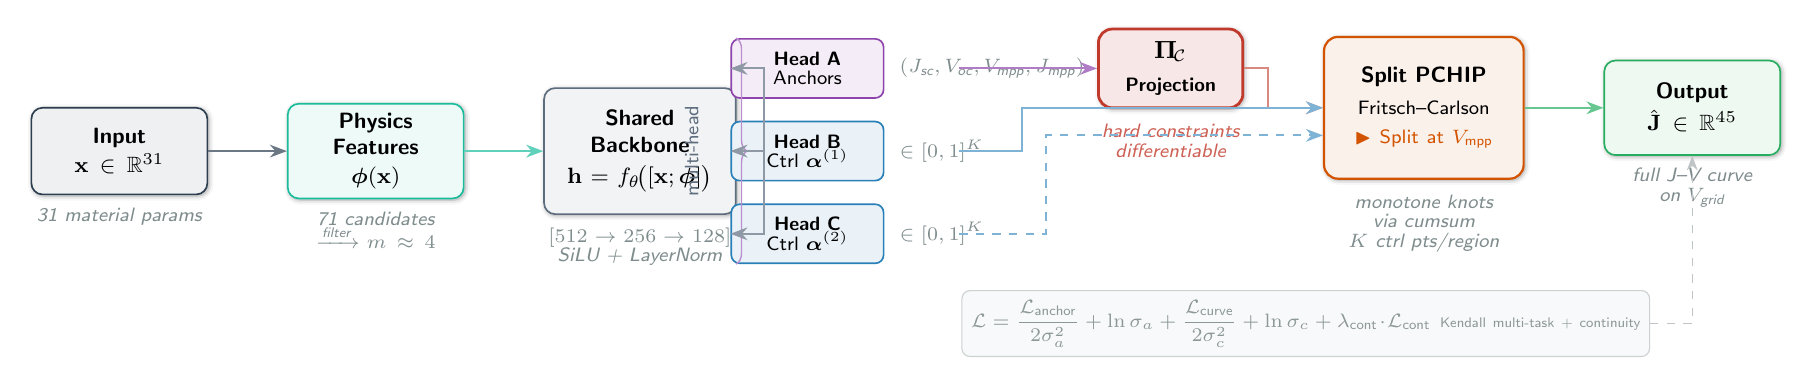
\begin{tikzpicture}[
  >=Stealth,
  every node/.style={font=\sffamily\small},
  block/.style={
    draw=#1, fill=#1!8, rounded corners=4pt,
    minimum height=1.1cm, text width=2.0cm, align=center,
    line width=0.6pt, font=\sffamily\footnotesize,
    blur shadow={shadow blur steps=3, shadow xshift=0.5pt, shadow yshift=-0.5pt}
  },
  headblock/.style={
    draw=#1, fill=#1!10, rounded corners=3pt,
    minimum height=0.75cm, text width=1.7cm, align=center,
    line width=0.6pt, font=\sffamily\scriptsize
  },
  arrow/.style={->, line width=0.7pt, color=#1},
  annot/.style={font=\sffamily\scriptsize\itshape, text=annotgray},
  brace/.style={decorate, decoration={brace, amplitude=4pt, raise=2pt}, line width=0.5pt},
]

% ═══════════════════════════════════════════
% INPUT BLOCK
% ═══════════════════════════════════════════
\node[block=inputblue] (input) {
  \textbf{Input}\\[1pt]
  $\mathbf{x}\in\mathbb{R}^{31}$
};

\node[annot, below=1pt of input] {31 material params};

% ═══════════════════════════════════════════
% PHYSICS FEATURE GENERATOR
% ═══════════════════════════════════════════
\node[block=featureteal, right=1.0cm of input] (features) {
  \textbf{Physics}\\
  \textbf{Features}\\[1pt]
  $\boldsymbol{\phi}(\mathbf{x})$
};

\node[annot, below=1pt of features, text width=2.2cm, align=center] {
  71 candidates\\[-1pt]
  $\xrightarrow{\text{filter}}$ $m \approx 4$
};

% ═══════════════════════════════════════════
% SHARED BACKBONE
% ═══════════════════════════════════════════
\node[block=backbonegray, right=1.0cm of features, minimum height=1.6cm, text width=2.2cm] (backbone) {
  \textbf{Shared}\\
  \textbf{Backbone}\\[2pt]
  $\mathbf{h} = f_\theta\!\bigl([\mathbf{x};\boldsymbol{\phi}]\bigr)$
};

\node[annot, below=1pt of backbone, text width=2.4cm, align=center] {
  $[512 \to 256 \to 128]$\\[-1pt]
  SiLU + LayerNorm
};

% ═══════════════════════════════════════════
% THREE HEADS
% ═══════════════════════════════════════════
\coordinate (headstart) at ($(backbone.east)+(0.9,0)$);

% Head A — Anchors
\node[headblock=headA] (headA) at ($(headstart)+(0, 1.05)$) {
  \textbf{Head A}\\[-1pt]
  Anchors
};

% Head B — Region 1
\node[headblock=headB] (headB) at ($(headstart)+(0, 0)$) {
  \textbf{Head B}\\[-1pt]
  Ctrl $\boldsymbol{\alpha}^{(1)}$
};

% Head C — Region 2
\node[headblock=headC] (headC) at ($(headstart)+(0,-1.05)$) {
  \textbf{Head C}\\[-1pt]
  Ctrl $\boldsymbol{\alpha}^{(2)}$
};

% Head annotations
\node[annot, right=2pt of headA.east, anchor=west] {
  $(J_{\text{sc}}, V_{\text{oc}}, V_{\text{mpp}}, J_{\text{mpp}})$
};
\node[annot, right=2pt of headB.east, anchor=west] {
  $\in [0,1]^K$
};
\node[annot, right=2pt of headC.east, anchor=west] {
  $\in [0,1]^K$
};

% Brace for heads
\draw[brace, headA!60] (headA.north west) -- (headC.south west)
  node[midway, left=8pt, font=\sffamily\scriptsize, text=backbonegray, rotate=90, anchor=south] {multi-head};

% ═══════════════════════════════════════════
% PROJECTION Π_C
% ═══════════════════════════════════════════
\node[
  draw=projred, fill=projred!12, rounded corners=5pt,
  minimum height=1.0cm, text width=1.6cm, align=center,
  line width=1.0pt, font=\sffamily\small,
  right=2.7cm of headA,
  blur shadow={shadow blur steps=3, shadow xshift=0.5pt, shadow yshift=-0.5pt}
] (proj) {
  $\boldsymbol{\Pi}_{\!\mathcal{C}}$\\[1pt]
  {\scriptsize\textbf{Projection}}
};

\node[annot, below=2pt of proj, text width=2.0cm, align=center, text=projred!80] {
  hard constraints\\[-1pt]
  differentiable
};

% ═══════════════════════════════════════════
% SPLIT PCHIP LAYER
% ═══════════════════════════════════════════
\node[
  draw=splineorg, fill=splineorg!8, rounded corners=5pt,
  minimum height=1.8cm, text width=2.3cm, align=center,
  line width=0.8pt, font=\sffamily\footnotesize,
  right=1.0cm of proj, yshift=-0.5cm,
  blur shadow={shadow blur steps=3, shadow xshift=0.5pt, shadow yshift=-0.5pt}
] (spline) {
  \textbf{Split PCHIP}\\[2pt]
  {\scriptsize Fritsch--Carlson}\\[1pt]
  {\scriptsize \textcolor{splineorg}{$\blacktriangleright$ Split at $V_{\text{mpp}}$}}
};

\node[annot, below=2pt of spline, text width=2.5cm, align=center] {
  monotone knots\\[-1pt]
  via cumsum\\[-1pt]
  $K$ ctrl pts/region
};

% ═══════════════════════════════════════════
% OUTPUT
% ═══════════════════════════════════════════
\node[block=outputgrn, right=1.0cm of spline, minimum height=1.2cm] (output) {
  \textbf{Output}\\[2pt]
  $\hat{\mathbf{J}}\in\mathbb{R}^{45}$
};

\node[annot, below=1pt of output, text width=2.2cm, align=center] {
  full J--V curve\\[-1pt]
  on $V_{\text{grid}}$
};

% ═══════════════════════════════════════════
% ARROWS — main dataflow
% ═══════════════════════════════════════════
\draw[arrow=inputblue!70] (input) -- (features);
\draw[arrow=featureteal!70] (features) -- (backbone);

% Backbone to heads
\draw[arrow=backbonegray!70] (backbone.east) -- ++(0.35,0) |- (headA.west);
\draw[arrow=backbonegray!70] (backbone.east) -- ++(0.35,0) |- (headB.west);
\draw[arrow=backbonegray!70] (backbone.east) -- ++(0.35,0) |- (headC.west);

% Head A to projection
\draw[arrow=headA!70] ($(headA.east)+(0.95,0)$) -- (proj.west);

% Projection to spline
\draw[arrow=projred!60] (proj.east) -- ++(0.3,0) |- (spline.west);

% Head B,C to spline
\draw[arrow=headB!60] ($(headB.east)+(0.95,0)$) -- ++(0.8,0) |- ($(spline.west)+(0,0.0)$);
\draw[arrow=headC!60, dashed] ($(headC.east)+(0.95,0)$) -- ++(1.1,0) |- ($(spline.west)+(0,-0.35)$);

% Spline to output
\draw[arrow=outputgrn!70] (spline.east) -- (output.west);

% ═══════════════════════════════════════════
% LOSS ANNOTATION (bottom)
% ═══════════════════════════════════════════
\node[
  draw=annotgray!40, fill=bgcard, rounded corners=3pt,
  font=\sffamily\scriptsize, text=annotgray!90,
  text width=8.5cm, align=left,
  below=1.4cm of spline, xshift=-1.5cm
] (lossbox) {
  $\mathcal{L} = \dfrac{\mathcal{L}_{\text{anchor}}}{2\sigma_a^2}
  + \ln\sigma_a
  + \dfrac{\mathcal{L}_{\text{curve}}}{2\sigma_c^2}
  + \ln\sigma_c
  + \lambda_{\text{cont}}\!\cdot\!\mathcal{L}_{\text{cont}}$
  \hfill {\tiny Kendall multi-task + continuity}
};

% Dashed line from loss to output
\draw[dashed, annotgray!50, line width=0.5pt, ->] (lossbox.east) -| ($(output.south)+(0,0)$);

\end{tikzpicture}
\end{document}
 (without \documentclass wrapper)
\documentclass[border=8pt]{standalone}
\usepackage{tikz}
\usepackage{amsmath,amssymb}
\usetikzlibrary{
  arrows.meta,
  calc,
  positioning,
  decorations.pathreplacing,
  fit,
  backgrounds,
  shadows.blur,
  shapes.geometric,
  patterns
}

% ── Colour palette (monochrome + accent) ──
\definecolor{inputblue}{HTML}{2C3E50}
\definecolor{featureteal}{HTML}{1ABC9C}
\definecolor{backbonegray}{HTML}{5D6D7E}
\definecolor{headA}{HTML}{8E44AD}
\definecolor{headB}{HTML}{2980B9}
\definecolor{headC}{HTML}{2980B9}
\definecolor{projred}{HTML}{C0392B}
\definecolor{splineorg}{HTML}{D35400}
\definecolor{outputgrn}{HTML}{27AE60}
\definecolor{bgcard}{HTML}{F8F9FA}
\definecolor{annotgray}{HTML}{7F8C8D}

\begin{document}
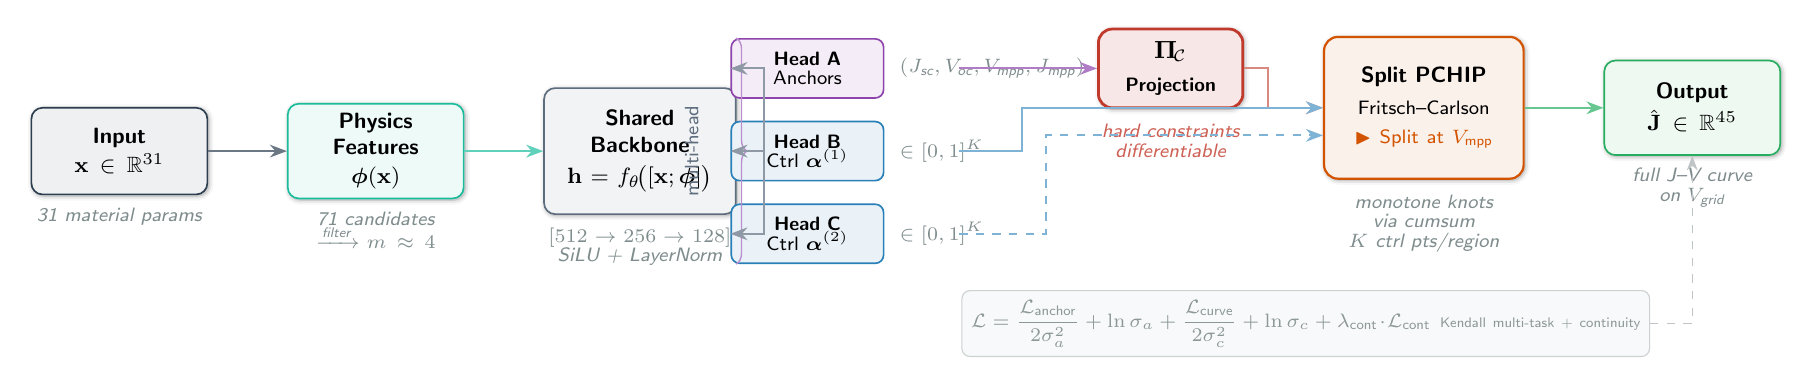
\begin{tikzpicture}[
  >=Stealth,
  every node/.style={font=\sffamily\small},
  block/.style={
    draw=#1, fill=#1!8, rounded corners=4pt,
    minimum height=1.1cm, text width=2.0cm, align=center,
    line width=0.6pt, font=\sffamily\footnotesize,
    blur shadow={shadow blur steps=3, shadow xshift=0.5pt, shadow yshift=-0.5pt}
  },
  headblock/.style={
    draw=#1, fill=#1!10, rounded corners=3pt,
    minimum height=0.75cm, text width=1.7cm, align=center,
    line width=0.6pt, font=\sffamily\scriptsize
  },
  arrow/.style={->, line width=0.7pt, color=#1},
  annot/.style={font=\sffamily\scriptsize\itshape, text=annotgray},
  brace/.style={decorate, decoration={brace, amplitude=4pt, raise=2pt}, line width=0.5pt},
]

% ═══════════════════════════════════════════
% INPUT BLOCK
% ═══════════════════════════════════════════
\node[block=inputblue] (input) {
  \textbf{Input}\\[1pt]
  $\mathbf{x}\in\mathbb{R}^{31}$
};

\node[annot, below=1pt of input] {31 material params};

% ═══════════════════════════════════════════
% PHYSICS FEATURE GENERATOR
% ═══════════════════════════════════════════
\node[block=featureteal, right=1.0cm of input] (features) {
  \textbf{Physics}\\
  \textbf{Features}\\[1pt]
  $\boldsymbol{\phi}(\mathbf{x})$
};

\node[annot, below=1pt of features, text width=2.2cm, align=center] {
  71 candidates\\[-1pt]
  $\xrightarrow{\text{filter}}$ $m \approx 4$
};

% ═══════════════════════════════════════════
% SHARED BACKBONE
% ═══════════════════════════════════════════
\node[block=backbonegray, right=1.0cm of features, minimum height=1.6cm, text width=2.2cm] (backbone) {
  \textbf{Shared}\\
  \textbf{Backbone}\\[2pt]
  $\mathbf{h} = f_\theta\!\bigl([\mathbf{x};\boldsymbol{\phi}]\bigr)$
};

\node[annot, below=1pt of backbone, text width=2.4cm, align=center] {
  $[512 \to 256 \to 128]$\\[-1pt]
  SiLU + LayerNorm
};

% ═══════════════════════════════════════════
% THREE HEADS
% ═══════════════════════════════════════════
\coordinate (headstart) at ($(backbone.east)+(0.9,0)$);

% Head A — Anchors
\node[headblock=headA] (headA) at ($(headstart)+(0, 1.05)$) {
  \textbf{Head A}\\[-1pt]
  Anchors
};

% Head B — Region 1
\node[headblock=headB] (headB) at ($(headstart)+(0, 0)$) {
  \textbf{Head B}\\[-1pt]
  Ctrl $\boldsymbol{\alpha}^{(1)}$
};

% Head C — Region 2
\node[headblock=headC] (headC) at ($(headstart)+(0,-1.05)$) {
  \textbf{Head C}\\[-1pt]
  Ctrl $\boldsymbol{\alpha}^{(2)}$
};

% Head annotations
\node[annot, right=2pt of headA.east, anchor=west] {
  $(J_{\text{sc}}, V_{\text{oc}}, V_{\text{mpp}}, J_{\text{mpp}})$
};
\node[annot, right=2pt of headB.east, anchor=west] {
  $\in [0,1]^K$
};
\node[annot, right=2pt of headC.east, anchor=west] {
  $\in [0,1]^K$
};

% Brace for heads
\draw[brace, headA!60] (headA.north west) -- (headC.south west)
  node[midway, left=8pt, font=\sffamily\scriptsize, text=backbonegray, rotate=90, anchor=south] {multi-head};

% ═══════════════════════════════════════════
% PROJECTION Π_C
% ═══════════════════════════════════════════
\node[
  draw=projred, fill=projred!12, rounded corners=5pt,
  minimum height=1.0cm, text width=1.6cm, align=center,
  line width=1.0pt, font=\sffamily\small,
  right=2.7cm of headA,
  blur shadow={shadow blur steps=3, shadow xshift=0.5pt, shadow yshift=-0.5pt}
] (proj) {
  $\boldsymbol{\Pi}_{\!\mathcal{C}}$\\[1pt]
  {\scriptsize\textbf{Projection}}
};

\node[annot, below=2pt of proj, text width=2.0cm, align=center, text=projred!80] {
  hard constraints\\[-1pt]
  differentiable
};

% ═══════════════════════════════════════════
% SPLIT PCHIP LAYER
% ═══════════════════════════════════════════
\node[
  draw=splineorg, fill=splineorg!8, rounded corners=5pt,
  minimum height=1.8cm, text width=2.3cm, align=center,
  line width=0.8pt, font=\sffamily\footnotesize,
  right=1.0cm of proj, yshift=-0.5cm,
  blur shadow={shadow blur steps=3, shadow xshift=0.5pt, shadow yshift=-0.5pt}
] (spline) {
  \textbf{Split PCHIP}\\[2pt]
  {\scriptsize Fritsch--Carlson}\\[1pt]
  {\scriptsize \textcolor{splineorg}{$\blacktriangleright$ Split at $V_{\text{mpp}}$}}
};

\node[annot, below=2pt of spline, text width=2.5cm, align=center] {
  monotone knots\\[-1pt]
  via cumsum\\[-1pt]
  $K$ ctrl pts/region
};

% ═══════════════════════════════════════════
% OUTPUT
% ═══════════════════════════════════════════
\node[block=outputgrn, right=1.0cm of spline, minimum height=1.2cm] (output) {
  \textbf{Output}\\[2pt]
  $\hat{\mathbf{J}}\in\mathbb{R}^{45}$
};

\node[annot, below=1pt of output, text width=2.2cm, align=center] {
  full J--V curve\\[-1pt]
  on $V_{\text{grid}}$
};

% ═══════════════════════════════════════════
% ARROWS — main dataflow
% ═══════════════════════════════════════════
\draw[arrow=inputblue!70] (input) -- (features);
\draw[arrow=featureteal!70] (features) -- (backbone);

% Backbone to heads
\draw[arrow=backbonegray!70] (backbone.east) -- ++(0.35,0) |- (headA.west);
\draw[arrow=backbonegray!70] (backbone.east) -- ++(0.35,0) |- (headB.west);
\draw[arrow=backbonegray!70] (backbone.east) -- ++(0.35,0) |- (headC.west);

% Head A to projection
\draw[arrow=headA!70] ($(headA.east)+(0.95,0)$) -- (proj.west);

% Projection to spline
\draw[arrow=projred!60] (proj.east) -- ++(0.3,0) |- (spline.west);

% Head B,C to spline
\draw[arrow=headB!60] ($(headB.east)+(0.95,0)$) -- ++(0.8,0) |- ($(spline.west)+(0,0.0)$);
\draw[arrow=headC!60, dashed] ($(headC.east)+(0.95,0)$) -- ++(1.1,0) |- ($(spline.west)+(0,-0.35)$);

% Spline to output
\draw[arrow=outputgrn!70] (spline.east) -- (output.west);

% ═══════════════════════════════════════════
% LOSS ANNOTATION (bottom)
% ═══════════════════════════════════════════
\node[
  draw=annotgray!40, fill=bgcard, rounded corners=3pt,
  font=\sffamily\scriptsize, text=annotgray!90,
  text width=8.5cm, align=left,
  below=1.4cm of spline, xshift=-1.5cm
] (lossbox) {
  $\mathcal{L} = \dfrac{\mathcal{L}_{\text{anchor}}}{2\sigma_a^2}
  + \ln\sigma_a
  + \dfrac{\mathcal{L}_{\text{curve}}}{2\sigma_c^2}
  + \ln\sigma_c
  + \lambda_{\text{cont}}\!\cdot\!\mathcal{L}_{\text{cont}}$
  \hfill {\tiny Kendall multi-task + continuity}
};

% Dashed line from loss to output
\draw[dashed, annotgray!50, line width=0.5pt, ->] (lossbox.east) -| ($(output.south)+(0,0)$);

\end{tikzpicture}
\end{document}
 (without \documentclass wrapper)
\documentclass[border=8pt]{standalone}
\usepackage{tikz}
\usepackage{amsmath,amssymb}
\usetikzlibrary{
  arrows.meta,
  calc,
  positioning,
  decorations.pathreplacing,
  fit,
  backgrounds,
  shadows.blur,
  shapes.geometric,
  patterns
}

% ── Colour palette (monochrome + accent) ──
\definecolor{inputblue}{HTML}{2C3E50}
\definecolor{featureteal}{HTML}{1ABC9C}
\definecolor{backbonegray}{HTML}{5D6D7E}
\definecolor{headA}{HTML}{8E44AD}
\definecolor{headB}{HTML}{2980B9}
\definecolor{headC}{HTML}{2980B9}
\definecolor{projred}{HTML}{C0392B}
\definecolor{splineorg}{HTML}{D35400}
\definecolor{outputgrn}{HTML}{27AE60}
\definecolor{bgcard}{HTML}{F8F9FA}
\definecolor{annotgray}{HTML}{7F8C8D}

\begin{document}
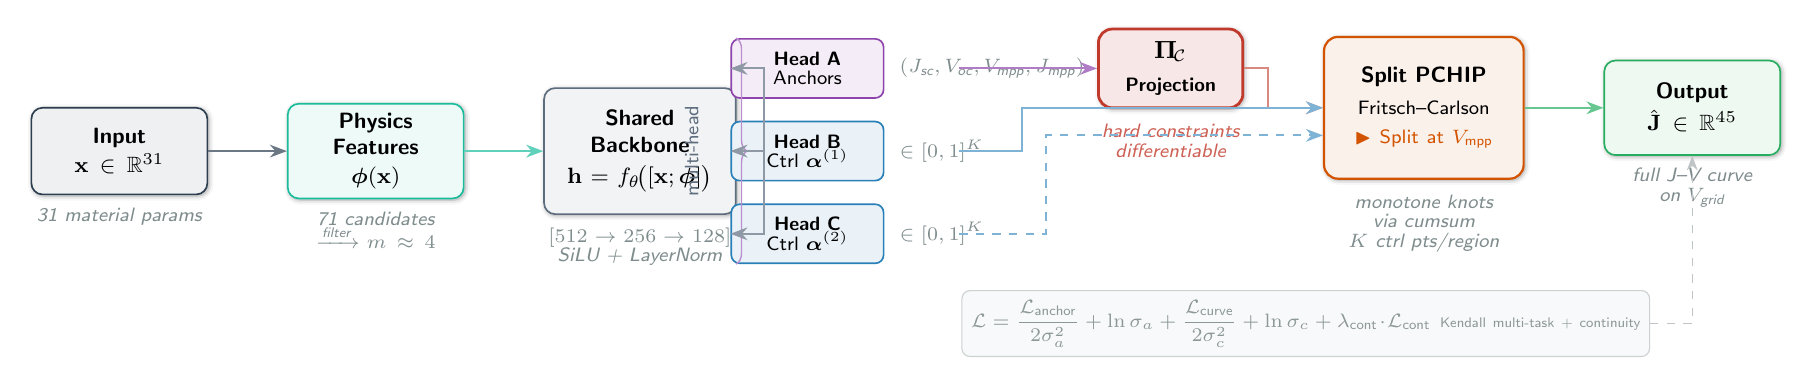
\begin{tikzpicture}[
  >=Stealth,
  every node/.style={font=\sffamily\small},
  block/.style={
    draw=#1, fill=#1!8, rounded corners=4pt,
    minimum height=1.1cm, text width=2.0cm, align=center,
    line width=0.6pt, font=\sffamily\footnotesize,
    blur shadow={shadow blur steps=3, shadow xshift=0.5pt, shadow yshift=-0.5pt}
  },
  headblock/.style={
    draw=#1, fill=#1!10, rounded corners=3pt,
    minimum height=0.75cm, text width=1.7cm, align=center,
    line width=0.6pt, font=\sffamily\scriptsize
  },
  arrow/.style={->, line width=0.7pt, color=#1},
  annot/.style={font=\sffamily\scriptsize\itshape, text=annotgray},
  brace/.style={decorate, decoration={brace, amplitude=4pt, raise=2pt}, line width=0.5pt},
]

% ═══════════════════════════════════════════
% INPUT BLOCK
% ═══════════════════════════════════════════
\node[block=inputblue] (input) {
  \textbf{Input}\\[1pt]
  $\mathbf{x}\in\mathbb{R}^{31}$
};

\node[annot, below=1pt of input] {31 material params};

% ═══════════════════════════════════════════
% PHYSICS FEATURE GENERATOR
% ═══════════════════════════════════════════
\node[block=featureteal, right=1.0cm of input] (features) {
  \textbf{Physics}\\
  \textbf{Features}\\[1pt]
  $\boldsymbol{\phi}(\mathbf{x})$
};

\node[annot, below=1pt of features, text width=2.2cm, align=center] {
  71 candidates\\[-1pt]
  $\xrightarrow{\text{filter}}$ $m \approx 4$
};

% ═══════════════════════════════════════════
% SHARED BACKBONE
% ═══════════════════════════════════════════
\node[block=backbonegray, right=1.0cm of features, minimum height=1.6cm, text width=2.2cm] (backbone) {
  \textbf{Shared}\\
  \textbf{Backbone}\\[2pt]
  $\mathbf{h} = f_\theta\!\bigl([\mathbf{x};\boldsymbol{\phi}]\bigr)$
};

\node[annot, below=1pt of backbone, text width=2.4cm, align=center] {
  $[512 \to 256 \to 128]$\\[-1pt]
  SiLU + LayerNorm
};

% ═══════════════════════════════════════════
% THREE HEADS
% ═══════════════════════════════════════════
\coordinate (headstart) at ($(backbone.east)+(0.9,0)$);

% Head A — Anchors
\node[headblock=headA] (headA) at ($(headstart)+(0, 1.05)$) {
  \textbf{Head A}\\[-1pt]
  Anchors
};

% Head B — Region 1
\node[headblock=headB] (headB) at ($(headstart)+(0, 0)$) {
  \textbf{Head B}\\[-1pt]
  Ctrl $\boldsymbol{\alpha}^{(1)}$
};

% Head C — Region 2
\node[headblock=headC] (headC) at ($(headstart)+(0,-1.05)$) {
  \textbf{Head C}\\[-1pt]
  Ctrl $\boldsymbol{\alpha}^{(2)}$
};

% Head annotations
\node[annot, right=2pt of headA.east, anchor=west] {
  $(J_{\text{sc}}, V_{\text{oc}}, V_{\text{mpp}}, J_{\text{mpp}})$
};
\node[annot, right=2pt of headB.east, anchor=west] {
  $\in [0,1]^K$
};
\node[annot, right=2pt of headC.east, anchor=west] {
  $\in [0,1]^K$
};

% Brace for heads
\draw[brace, headA!60] (headA.north west) -- (headC.south west)
  node[midway, left=8pt, font=\sffamily\scriptsize, text=backbonegray, rotate=90, anchor=south] {multi-head};

% ═══════════════════════════════════════════
% PROJECTION Π_C
% ═══════════════════════════════════════════
\node[
  draw=projred, fill=projred!12, rounded corners=5pt,
  minimum height=1.0cm, text width=1.6cm, align=center,
  line width=1.0pt, font=\sffamily\small,
  right=2.7cm of headA,
  blur shadow={shadow blur steps=3, shadow xshift=0.5pt, shadow yshift=-0.5pt}
] (proj) {
  $\boldsymbol{\Pi}_{\!\mathcal{C}}$\\[1pt]
  {\scriptsize\textbf{Projection}}
};

\node[annot, below=2pt of proj, text width=2.0cm, align=center, text=projred!80] {
  hard constraints\\[-1pt]
  differentiable
};

% ═══════════════════════════════════════════
% SPLIT PCHIP LAYER
% ═══════════════════════════════════════════
\node[
  draw=splineorg, fill=splineorg!8, rounded corners=5pt,
  minimum height=1.8cm, text width=2.3cm, align=center,
  line width=0.8pt, font=\sffamily\footnotesize,
  right=1.0cm of proj, yshift=-0.5cm,
  blur shadow={shadow blur steps=3, shadow xshift=0.5pt, shadow yshift=-0.5pt}
] (spline) {
  \textbf{Split PCHIP}\\[2pt]
  {\scriptsize Fritsch--Carlson}\\[1pt]
  {\scriptsize \textcolor{splineorg}{$\blacktriangleright$ Split at $V_{\text{mpp}}$}}
};

\node[annot, below=2pt of spline, text width=2.5cm, align=center] {
  monotone knots\\[-1pt]
  via cumsum\\[-1pt]
  $K$ ctrl pts/region
};

% ═══════════════════════════════════════════
% OUTPUT
% ═══════════════════════════════════════════
\node[block=outputgrn, right=1.0cm of spline, minimum height=1.2cm] (output) {
  \textbf{Output}\\[2pt]
  $\hat{\mathbf{J}}\in\mathbb{R}^{45}$
};

\node[annot, below=1pt of output, text width=2.2cm, align=center] {
  full J--V curve\\[-1pt]
  on $V_{\text{grid}}$
};

% ═══════════════════════════════════════════
% ARROWS — main dataflow
% ═══════════════════════════════════════════
\draw[arrow=inputblue!70] (input) -- (features);
\draw[arrow=featureteal!70] (features) -- (backbone);

% Backbone to heads
\draw[arrow=backbonegray!70] (backbone.east) -- ++(0.35,0) |- (headA.west);
\draw[arrow=backbonegray!70] (backbone.east) -- ++(0.35,0) |- (headB.west);
\draw[arrow=backbonegray!70] (backbone.east) -- ++(0.35,0) |- (headC.west);

% Head A to projection
\draw[arrow=headA!70] ($(headA.east)+(0.95,0)$) -- (proj.west);

% Projection to spline
\draw[arrow=projred!60] (proj.east) -- ++(0.3,0) |- (spline.west);

% Head B,C to spline
\draw[arrow=headB!60] ($(headB.east)+(0.95,0)$) -- ++(0.8,0) |- ($(spline.west)+(0,0.0)$);
\draw[arrow=headC!60, dashed] ($(headC.east)+(0.95,0)$) -- ++(1.1,0) |- ($(spline.west)+(0,-0.35)$);

% Spline to output
\draw[arrow=outputgrn!70] (spline.east) -- (output.west);

% ═══════════════════════════════════════════
% LOSS ANNOTATION (bottom)
% ═══════════════════════════════════════════
\node[
  draw=annotgray!40, fill=bgcard, rounded corners=3pt,
  font=\sffamily\scriptsize, text=annotgray!90,
  text width=8.5cm, align=left,
  below=1.4cm of spline, xshift=-1.5cm
] (lossbox) {
  $\mathcal{L} = \dfrac{\mathcal{L}_{\text{anchor}}}{2\sigma_a^2}
  + \ln\sigma_a
  + \dfrac{\mathcal{L}_{\text{curve}}}{2\sigma_c^2}
  + \ln\sigma_c
  + \lambda_{\text{cont}}\!\cdot\!\mathcal{L}_{\text{cont}}$
  \hfill {\tiny Kendall multi-task + continuity}
};

% Dashed line from loss to output
\draw[dashed, annotgray!50, line width=0.5pt, ->] (lossbox.east) -| ($(output.south)+(0,0)$);

\end{tikzpicture}
\end{document}
 (without \documentclass wrapper)
\documentclass[border=8pt]{standalone}
\usepackage{tikz}
\usepackage{amsmath,amssymb}
\usetikzlibrary{
  arrows.meta,
  calc,
  positioning,
  decorations.pathreplacing,
  fit,
  backgrounds,
  shadows.blur,
  shapes.geometric,
  patterns
}

% ── Colour palette (monochrome + accent) ──
\definecolor{inputblue}{HTML}{2C3E50}
\definecolor{featureteal}{HTML}{1ABC9C}
\definecolor{backbonegray}{HTML}{5D6D7E}
\definecolor{headA}{HTML}{8E44AD}
\definecolor{headB}{HTML}{2980B9}
\definecolor{headC}{HTML}{2980B9}
\definecolor{projred}{HTML}{C0392B}
\definecolor{splineorg}{HTML}{D35400}
\definecolor{outputgrn}{HTML}{27AE60}
\definecolor{bgcard}{HTML}{F8F9FA}
\definecolor{annotgray}{HTML}{7F8C8D}

\begin{document}
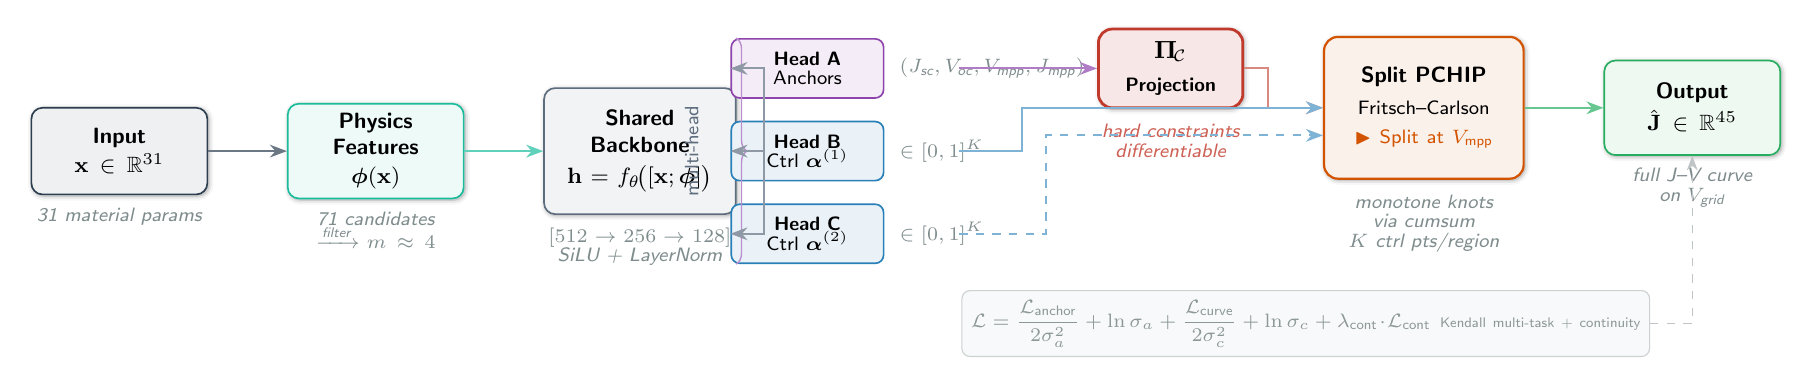
\begin{tikzpicture}[
  >=Stealth,
  every node/.style={font=\sffamily\small},
  block/.style={
    draw=#1, fill=#1!8, rounded corners=4pt,
    minimum height=1.1cm, text width=2.0cm, align=center,
    line width=0.6pt, font=\sffamily\footnotesize,
    blur shadow={shadow blur steps=3, shadow xshift=0.5pt, shadow yshift=-0.5pt}
  },
  headblock/.style={
    draw=#1, fill=#1!10, rounded corners=3pt,
    minimum height=0.75cm, text width=1.7cm, align=center,
    line width=0.6pt, font=\sffamily\scriptsize
  },
  arrow/.style={->, line width=0.7pt, color=#1},
  annot/.style={font=\sffamily\scriptsize\itshape, text=annotgray},
  brace/.style={decorate, decoration={brace, amplitude=4pt, raise=2pt}, line width=0.5pt},
]

% ═══════════════════════════════════════════
% INPUT BLOCK
% ═══════════════════════════════════════════
\node[block=inputblue] (input) {
  \textbf{Input}\\[1pt]
  $\mathbf{x}\in\mathbb{R}^{31}$
};

\node[annot, below=1pt of input] {31 material params};

% ═══════════════════════════════════════════
% PHYSICS FEATURE GENERATOR
% ═══════════════════════════════════════════
\node[block=featureteal, right=1.0cm of input] (features) {
  \textbf{Physics}\\
  \textbf{Features}\\[1pt]
  $\boldsymbol{\phi}(\mathbf{x})$
};

\node[annot, below=1pt of features, text width=2.2cm, align=center] {
  71 candidates\\[-1pt]
  $\xrightarrow{\text{filter}}$ $m \approx 4$
};

% ═══════════════════════════════════════════
% SHARED BACKBONE
% ═══════════════════════════════════════════
\node[block=backbonegray, right=1.0cm of features, minimum height=1.6cm, text width=2.2cm] (backbone) {
  \textbf{Shared}\\
  \textbf{Backbone}\\[2pt]
  $\mathbf{h} = f_\theta\!\bigl([\mathbf{x};\boldsymbol{\phi}]\bigr)$
};

\node[annot, below=1pt of backbone, text width=2.4cm, align=center] {
  $[512 \to 256 \to 128]$\\[-1pt]
  SiLU + LayerNorm
};

% ═══════════════════════════════════════════
% THREE HEADS
% ═══════════════════════════════════════════
\coordinate (headstart) at ($(backbone.east)+(0.9,0)$);

% Head A — Anchors
\node[headblock=headA] (headA) at ($(headstart)+(0, 1.05)$) {
  \textbf{Head A}\\[-1pt]
  Anchors
};

% Head B — Region 1
\node[headblock=headB] (headB) at ($(headstart)+(0, 0)$) {
  \textbf{Head B}\\[-1pt]
  Ctrl $\boldsymbol{\alpha}^{(1)}$
};

% Head C — Region 2
\node[headblock=headC] (headC) at ($(headstart)+(0,-1.05)$) {
  \textbf{Head C}\\[-1pt]
  Ctrl $\boldsymbol{\alpha}^{(2)}$
};

% Head annotations
\node[annot, right=2pt of headA.east, anchor=west] {
  $(J_{\text{sc}}, V_{\text{oc}}, V_{\text{mpp}}, J_{\text{mpp}})$
};
\node[annot, right=2pt of headB.east, anchor=west] {
  $\in [0,1]^K$
};
\node[annot, right=2pt of headC.east, anchor=west] {
  $\in [0,1]^K$
};

% Brace for heads
\draw[brace, headA!60] (headA.north west) -- (headC.south west)
  node[midway, left=8pt, font=\sffamily\scriptsize, text=backbonegray, rotate=90, anchor=south] {multi-head};

% ═══════════════════════════════════════════
% PROJECTION Π_C
% ═══════════════════════════════════════════
\node[
  draw=projred, fill=projred!12, rounded corners=5pt,
  minimum height=1.0cm, text width=1.6cm, align=center,
  line width=1.0pt, font=\sffamily\small,
  right=2.7cm of headA,
  blur shadow={shadow blur steps=3, shadow xshift=0.5pt, shadow yshift=-0.5pt}
] (proj) {
  $\boldsymbol{\Pi}_{\!\mathcal{C}}$\\[1pt]
  {\scriptsize\textbf{Projection}}
};

\node[annot, below=2pt of proj, text width=2.0cm, align=center, text=projred!80] {
  hard constraints\\[-1pt]
  differentiable
};

% ═══════════════════════════════════════════
% SPLIT PCHIP LAYER
% ═══════════════════════════════════════════
\node[
  draw=splineorg, fill=splineorg!8, rounded corners=5pt,
  minimum height=1.8cm, text width=2.3cm, align=center,
  line width=0.8pt, font=\sffamily\footnotesize,
  right=1.0cm of proj, yshift=-0.5cm,
  blur shadow={shadow blur steps=3, shadow xshift=0.5pt, shadow yshift=-0.5pt}
] (spline) {
  \textbf{Split PCHIP}\\[2pt]
  {\scriptsize Fritsch--Carlson}\\[1pt]
  {\scriptsize \textcolor{splineorg}{$\blacktriangleright$ Split at $V_{\text{mpp}}$}}
};

\node[annot, below=2pt of spline, text width=2.5cm, align=center] {
  monotone knots\\[-1pt]
  via cumsum\\[-1pt]
  $K$ ctrl pts/region
};

% ═══════════════════════════════════════════
% OUTPUT
% ═══════════════════════════════════════════
\node[block=outputgrn, right=1.0cm of spline, minimum height=1.2cm] (output) {
  \textbf{Output}\\[2pt]
  $\hat{\mathbf{J}}\in\mathbb{R}^{45}$
};

\node[annot, below=1pt of output, text width=2.2cm, align=center] {
  full J--V curve\\[-1pt]
  on $V_{\text{grid}}$
};

% ═══════════════════════════════════════════
% ARROWS — main dataflow
% ═══════════════════════════════════════════
\draw[arrow=inputblue!70] (input) -- (features);
\draw[arrow=featureteal!70] (features) -- (backbone);

% Backbone to heads
\draw[arrow=backbonegray!70] (backbone.east) -- ++(0.35,0) |- (headA.west);
\draw[arrow=backbonegray!70] (backbone.east) -- ++(0.35,0) |- (headB.west);
\draw[arrow=backbonegray!70] (backbone.east) -- ++(0.35,0) |- (headC.west);

% Head A to projection
\draw[arrow=headA!70] ($(headA.east)+(0.95,0)$) -- (proj.west);

% Projection to spline
\draw[arrow=projred!60] (proj.east) -- ++(0.3,0) |- (spline.west);

% Head B,C to spline
\draw[arrow=headB!60] ($(headB.east)+(0.95,0)$) -- ++(0.8,0) |- ($(spline.west)+(0,0.0)$);
\draw[arrow=headC!60, dashed] ($(headC.east)+(0.95,0)$) -- ++(1.1,0) |- ($(spline.west)+(0,-0.35)$);

% Spline to output
\draw[arrow=outputgrn!70] (spline.east) -- (output.west);

% ═══════════════════════════════════════════
% LOSS ANNOTATION (bottom)
% ═══════════════════════════════════════════
\node[
  draw=annotgray!40, fill=bgcard, rounded corners=3pt,
  font=\sffamily\scriptsize, text=annotgray!90,
  text width=8.5cm, align=left,
  below=1.4cm of spline, xshift=-1.5cm
] (lossbox) {
  $\mathcal{L} = \dfrac{\mathcal{L}_{\text{anchor}}}{2\sigma_a^2}
  + \ln\sigma_a
  + \dfrac{\mathcal{L}_{\text{curve}}}{2\sigma_c^2}
  + \ln\sigma_c
  + \lambda_{\text{cont}}\!\cdot\!\mathcal{L}_{\text{cont}}$
  \hfill {\tiny Kendall multi-task + continuity}
};

% Dashed line from loss to output
\draw[dashed, annotgray!50, line width=0.5pt, ->] (lossbox.east) -| ($(output.south)+(0,0)$);

\end{tikzpicture}
\end{document}
